%Begin


%%%%%%%%%%%%%%%%%%%%%%%%%%%%%%%%%%%%%%%%%%%%%%%%%%%%%%%%%%%%%%%
\chapter*{\S \space II. --- PRÉLIMINAIRES TOPOLOGIQUES~: SAUVAGERIE, DÉCOUPE}
\addcontentsline{toc}{section}{II. Préliminaires topologiques~: sauvagerie, découpe}
\section*{}

La première partie de ce chapitre est consacrée aux problèmes de ``sauvagerie'' liés aux plongements de 1-complexes dans les surfaces à bord. Dans une seconde partie, on introduit la notion de ``découpe d'une surface suivant un 1-complexe plongé'' (dans un cadre plus général)~; il s'agit d'un outil qui sera fort utile dans la suite.

%%%%%%%%%%%%%%%%%%%%%%%%%%%%%%%%%%%%
\subsection*{1. Terminologie.}
\addcontentsline{toc}{subsection}{1. Terminologie}

{\bf 1.1}. --- Nous appellerons \emph{surface} (resp. \emph{surface à bord}) toute $2$-variété topologique (resp. $2$-variété à bord topologique, le bord pouvant être vide). Si $X$ est une surface à bord, son bord sera noté $\partial X$~; lorsque $X$ est orientable, toute orientation de $X$ induit une orientation de $\partial X$ (cf. définitions classiques de l'orientation, par exemple dans [79], ou bien la définition équivalente donnée en {\bf 5.4.2.1.}). 

On appellera \emph{intérieur} de $X$ la surface $X \setminus \partial X$, et on la notera $\operatorname{int} X$.

On considèrera également des \emph{surfaces à bord généralisé}~: il s'agit de couples $(X, P)$, où $X$ est une surface à bord et $P$ est une partie finie de $\operatorname{int} X$~; le \emph{bord généralisé} de $(X, P)$ est alors $\partial'X = \partial X \amalg P$, \emph{l'intérieur} de $(X,P)$ est par définition $X \setminus \partial'X$. (Par abus de langage on parlera de la surface à bord généralisé $X$, du bord généralisé de $X$, de l'intérieur de $X$).

Une surface à bord $X$ orientable compacte et de genre $g$ (i.e~: nombre d'anses de la surface obtenue en recollant des disques sur les composantes de $\partial X$) telle que $\operatorname{card} \pi_0 \partial X = p$ sera dite de \emph{type} $(g,p)$ (les surfaces à bord orientables compactes sont classifiées à homéomorphisme près par leur type~: cf. [79]).

Nous appellerons \emph{disque} (resp. \emph{cylindre, bicouronne}) toute surface à bord de type $(0,1)$ (resp. $(0,2), (0,3)$).

Nous appellerons \emph{disque} (resp. \emph{cylindre, bicouronne}) \emph{de $X$} (où $X$ est une surface à bord) toute partie de $X$ qui est un disque (resp. cylindre, bicouronne) pour la topologie induite.

Nous noterons dans toute la suite $B(0;\rho)$ la boule fermée de centre $0$ et de rayon $\rho$ dans $\mathbf{R}^2$ (où $\rho$ est un nombre réel positif). Comme $\mathbf{R}^2$ est identifié canoniquement à l'ensemble $\mathbf{C}$ des nombres complexes, on désignera les points de $B(0;\rho)$ par des nombres complexes (de module inférieur ou égal à $\rho$). On considère dans la suite que $\mathbf{R}^2$ est orienté de façon standard. Par conséquent $B(0;1)$ est munie d'une orientation standard induite par celle de $\mathbf{R}^2$, et $\mathbb{S}^1$ (nombres complexes de module $1$) est munie d'une orientation standard induite par $B(0;1)$ (car $\mathbb{S}^1 = \partial B(0;1)$).

De même $I = [0,1]$ sera toujours considéré comme muni de l'orientation standard (induite par l'ordre).

\vskip .3cm
{\bf 1.2}. --- Nous appellerons \emph{courbe simple} (resp. \emph{arc simple}) \emph{dans $X$} (où $X$ est une surface à bord) l'image d'une application injective et continue de $\mathbb{S}^1$ (resp. $I$) dans $X$, c'est une $1$-variété (resp. $1$-variété à bord).

Lorsque $a$ et $b$ sont deux points d'un arc simple orienté ou d'une courbe simple orientée, on désignera par $[a,b]$ la partie fermée de cet arc, ou de cette courbe, comprise entre $a$ et $b$, en suivant l'orientation de $a$ vers $b$.

\vskip .3cm
{\bf 1.3}. --- Etant donné un $1$-complexe topologique compact $K$ et une surface à bord $X$, on appellera \emph{plongement} de $K$ dans $X$ toute injection continue de $K$ \emph{dans $\operatorname{int} X$}. (Cette notion s'étend immédiatement aux surfaces à bord généralisé).

\vskip .3cm
{\bf 1.4}. --- Si $X, Y$ sont deux surfaces orientées à bords et $h$ un homéomorphisme de $X$ sur $Y$, $h$ sera dit \emph{orienté} s'il conserve les orientations. Si $(X, A)$ et $(Y, B)$ sont deux couples d'espaces topologiques tels que~: $A \subset X$ et $B \subset Y$, par homéomorphisme $h$ du couple $(X, A)$ sur le couple $(Y, B)$ on entend un homéomorphisme de $X$ sur $Y$ induisant, par restriction à $A$, un homéomorphisme de $A$ sur $B$.

\vskip .3cm
{\bf 1.5}. --- Nous appellerons \emph{torseur} (à gauche) sous un groupe $G$, la donnée d'un ensemble $E$ et d'une opération (à gauche) de $G$ sur $E$ telle que $E$ soit un espace principal homogène sous $G$ (i.e. $E$ est non vide et~: $\forall (x,y) \in E \times E$ il existe un unique $g$ de $G$ tel que $g \cdot x = y$). 
$E$ est alors isomorphe (en tant qu'espace homogène) à l'espace homogène $G_g$ constitué par $G$ muni de l'opération par translations à gauche de $G$. 
Il en résulte que $\operatorname{Card} E = \operatorname{Card} G$. Le choix d'un élément $x_0$ de $E$ permet d'identifier $G_g$ à $E$ par la loi $g \to g \cdot x_0$.

\vskip .3cm
{\bf 1.6}. ---  Si $E$ est un ensemble fini tel que $\operatorname{Card} E = n$, un \emph{ordre circulaire} $\omega$ sur $E$ est la donnée d'une structure de $\mathbf{Z}/n\mathbf{Z}$ torseur sur $E$. Si, pour $x \in E$, $\bar{p} \in \mathbf{Z}/n\mathbf{Z}$, on note $\bar{p} + x$ le transformé de $x$ par $\bar{p}$, l'élément $\bar{1} + x$ sera appelé le \emph{suivant} de $x$ dans l'ordre circulaire $\omega$ et sera noté $\omega(x)$. Si $n \neq 1$, on a $\omega(x) \neq x$. Il y a $(n-1)!$ ordres circulaires distincts sur $E$.

Pour chaque $x \in E$ il existe un seul $y \in E$ tel que $\omega(y) = x$, $y$ sera appelé le \emph{précédent} de $x$, dans l'ordre circulaire $\omega$~; il existe un ordre circulaire $\omega'$ sur $E$ ($\omega'$ unique) tel que pour tout $x \in E$, $\omega'(x)$ soit le précédent de $x$ dans l'ordre circulaire $\omega$~; on dira que $\omega'$ est l'ordre circulaire \emph{inverse} de $\omega$ et on le notera $\omega^{-1}$.

Si $E$ est muni de l'ordre circulaire $\omega$, le choix d'un élément $a_0$ de $E$ permet d'identifier $E$ à $\mathbf{Z}/n\mathbf{Z}$ et on pourra ainsi noter $a_p$ ($p=0,1,\dots n-1$) l'élément $\bar{p} + a_0$ de $E$. On a alors $E = \{a_0, a_1, \dots, a_{n-1}\}$.

%%%%%%%%%%%%%%%%%%%%%%%%%%%%%%%%%%%%
\subsection*{2. Problèmes de sauvagerie.}
\addcontentsline{toc}{subsection}{2. Problèmes de sauvagerie}

Etant donné la définition choisie pour les plongements d'un $1$-complexe $K$ dans une surface à bord $X$, il nous faut d'abord vérifier, en vue de l'étude ultérieure, que si $i$ est un tel plongement, tout point de $i(K)$ possède un voisinage dans $X$ pour lequel il existe une \emph{``carte adaptée''} (i.e.~: dans laquelle, localement, le plongement est lu selon un plongement sur une étoile standard de $\mathbf{R}^2$). C'est l'objet des propositions de ce paragraphe et du suivant.

{\bf 2.1.} Nous utiliserons souvent le théorème suivant du à Shoenflies (cf. [1], [98])~:
\vskip .3cm
{
Théorème {\bf 2.1.1.} --- \it Toute injection continue de $\mathbb{S}^1$ dans $\mathbf{R}^2$ se prolonge en un homéomorphisme de $\mathbf{R}^2$ sur lui-même.
}
\vskip .3cm
Il en résulte qu'une telle injection continue est un plongement de variétés topologiques. Nous voulons un résultat ``analogue'' pour les $1$-complexes.

Un corollaire immédiat de ce théorème est le suivant~:
\vskip .3cm
{
Proposition {\bf 2.1.2.} --- \it Si $D$ est un disque et $\gamma$ une courbe simple dans $\operatorname{int} D$, alors la composante connexe de $D \setminus \gamma$ ne contenant pas $\partial D$ est un disque ouvert (appelé \textup{intérieur de $\gamma$ dans $D$}) dont la frontière est $\gamma$. Si $D'$ est un second disque et $\gamma'$ une courbe simple de $\operatorname{int} D'$, tout homéomorphisme de $\gamma$ sur $\gamma'$ peut être prolongé en un homéomorphisme de l'intérieur de $\gamma$ sur l'intérieur de $\gamma'$.
}
\vskip .3cm
{\bf 2.2.} Le lemme du segment.
\vskip .3cm
{
Proposition {\bf 2.2.1.} --- \it Toute injection continue de $I$ ($I = [0,1]$) dans $\mathbf{R}^2$ se prolonge en un homéomorphisme de $\mathbf{R}^2$ sur lui-même.
}
\vskip .3cm
Pour démontrer cette proposition nous utiliserons les deux lemmes suivants~:

\vskip .3cm
{
Lemme {\bf 2.2.2.} (Théorème de Janiszewski) (cf. [27], [98]). --- \it Soient $A$ un fermé de $\mathbf{R}^2$, $B$ un compact de $\mathbf{R}^2$, $a, b$ deux points distincts de $\mathbf{R}^2 \setminus (A \cup B)$. Si ni $A$ ni $B$ ne sépare $a$ et $b$, et si $A \cap B$ est connexe, alors $A \cup B$ ne sépare pas $a$ et $b$ (N.B~: une partie $P$ de $\mathbf{R}^2$ \textup{sépare} les points $a$ et $b$ si $a, b$ n'appartiennent pas à la même composante connexe par arcs de $\mathbf{R}^2 \setminus P$).
}
\vskip .3cm
{
Lemme {\bf 2.2.3.} (cf [27], [98]). --- \it Le complémentaire dans $\mathbf{R}^2$ d'un arc simple est connexe.
}
\vskip .3cm
{\bf 2.2.4.} On démontre alors~:
\vskip .3cm
{
Lemme de connexité. --- \it Soit $U$ un ouvert connexe de $\mathbf{R}^2$, $J$ un arc simple de $\mathbf{R}^2$ d'extrémités $a$ et $b$ tel que $J \setminus \{b\} \subset U$, alors $U \setminus J$ est un ouvert connexe de $\mathbf{R}^2$.
}
\vskip .3cm
Démonstration. Soit $A$ le complémentaire de $U$ dans $\mathbf{R}^2$, c'est un fermé de $\mathbf{R}^2$. Soit $B = J$, et soient $x$ et $y$ deux points distincts de $U \setminus J$. Alors, $A$ ne sépare pas $x$ et $y$ puisque $U$ est un ouvert connexe (et donc connexe par arcs). $B$ ne sépare pas $x$ et $y$ (lemme {\bf 2.2.3}). Le lemme 2.2.2 entraîne donc que $A \cup B = U \setminus J$ ne sépare pas $x$ et $y$~; $U \setminus J$ est donc connexe (par arcs).
\vskip .3cm
{
Lemme d'accessibilité {\bf 2.2.5.} --- \it Soit $U$ un ouvert connexe de $\mathbf{R}^2$, $J$ un arc simple de $\mathbf{R}^2$ d'extrémités $a$ et $b$ tel que $J \setminus \{b\} \subset U$, et soit $x$ un point quelconque de $U \setminus J$. On peut joindre $x$ à $a$ par un arc simple $J'$ avec $J' \setminus \{a\}$ contenu dans $U \setminus J$, et toute partie de $J'$ de la forme $[x, \alpha]$ ($\alpha \neq a$, $\alpha \in J'$) étant une réunion de segments.
}
\vskip .3cm
Démonstration. Soit $B_1$ une boule fermée de centre $a$, de rayon $\rho_1$ tel que $b \notin B_1$ et $B_1 \subset U$. Soit $b_1$ le premier point de $J$ qui soit sur la frontière $F_1$ de $B_1$ lorsqu'on décrit $J$ de $a$ vers $b$ ($b_1$ existe par compacité de $F_1$ et $J$). La portion d'arc $[a, b_1[$ est donc contenue dans $\operatorname{int} B_1$ (on note ainsi l'intérieur de $B_1$, qui est une boule ouverte). Soit $J_1$ l'arc $[b_1, b]$ : c'est un compact ; $\operatorname{int} B_1 \setminus J_1$ est ouvert, on note $U_1$ la composante connexe de cet ouvert qui contient $[a, b_1[$ ; $U_1$ est un ouvert connexe vérifiant, avec l'arc $[a, b_1]$, les hypothèses du lemme de connexité {\bf 2.2.4.}~: $U_1 \setminus [a, b_1[$ est donc connexe.

Soit $x_1$ un point de $U_1 \setminus [a, b_1[$ ; comme le complémentaire de $J$ dans $U$ est connexe par arcs (toujours à cause du lemme {\bf 2.2.4.}), on peut, dans ce complémentaire, joindre $x$ à $x_1$ par un arc simple linéaire par morceaux.

On itère alors l'opération précédente en remplaçant $U$ par $U_1$ et $J$ par $[a, b_1]$ : on choisit $B_2$, boule fermée de centre $a$ et de rayon $\rho_2$ tel que $\rho_2 \le \frac{\rho_1}{2}$, $B_2 \subset U_1$ et $\rho_2 < d(a, x_1)$. On appelle $b_2$ le premier point de $J$ qui soit sur $F_2$, la frontière de $B_2$ (lorsque $J$ est décrit de $a$ vers $b$). On construit $U_2$, comme précédemment $U_1$, et on choisit un point $x_2$ de $U_2 \setminus [a, b_2[$, on a $x_2 \in U_1$ et dans $U_1 \setminus J \cap U_1$, connexe par arcs, on joint $x_1$ à $x_2$ par un arc simple linéaire par morceau ne rencontrant pas $[x, x_1]$. En itérant cette opération on construit une suite d'arcs simples linéaires par morceaux : $[x, x_1], [x_1, x_2], \dots, [x_{n-1}, x_n], \dots$ L'ensemble obtenu en rajoutant à $a$ la réunion de ces arcs est un arc simple joignant $x$ à $a$ (la continuité en $a$ se déduit de ce que, pour tout entier $n$, $[x_n, x_{n-1}]$ est contenu dans la boule $B_n$ de rayon inférieur à $\frac{\rho_1}{2^n}$).
\vskip .3cm
{\bf 2.2.6.} Démonstration de la proposition 2.2.1.~:
Soit $i$ une injection continue de $I$ dans $\mathbf{R}^2$ et $J$ l'arc $i(I)$. Par le lemme 2.2.5. on peut prolonger $J$ en ses deux extrémités de façon à obtenir un arc $J'$ qui soit linéaire par morceau au voisinage des extrémités. Prenant un point $x$ de $\mathbf{R}^2 \setminus J'$, on peut alors joindre $x$ aux deux extrémités de $J'$ par deux arcs simples n'ayant que $x$ en commun. On obtient ainsi une courbe simple de $\mathbf{R}^2$, image d'une injection continue $\tilde{i}$ de $\partial(I \times I)$ dans $\mathbf{R}^2$, ($\tilde{i}|I = i$). Soit $\tilde{h}$ un homéomorphisme de $\mathbf{R}^2$ sur $\mathbf{R}^2$ tel que $\tilde{h}(\mathbb{S}^1) = \partial(I \times I)$ et soit $h = \tilde{h}|\mathbb{S}^1$. Alors, $\tilde{i} \circ h$ est une injection continue de $\mathbb{S}^1$ dans $\mathbf{R}^2$ et se prolonge ({\bf 2.1.1.}) en homéomorphisme $g$ de $\mathbf{R}^2$ sur lui-même~; $\tilde{h}^{-1} \circ g$ est un homéomorphisme de $\mathbf{R}^2$ sur $\mathbf{R}^2$, prolongeant $i$.
\vskip .3cm
{\bf 2.3.} Carte adaptée à un plongement en un point.

Soient $K$ un $1$-complexe compact, $X$ une surface à bord, et $i$ un plongement de $K$ dans $X$. Rappelons qu'on note $B(0;\rho)$ la boule fermée de $\mathbf{R}^2$ de centre $0$ et de rayon $\rho$. On définit \underline{l'étoile standard fermée à $n$ branches} $\overline{\St}_n$ comme étant l'adhérence de $\St_n$ dans $\mathbf{R}^2$.
\vskip .3cm
{
Théorème {\bf 2.3.1.} --- \it Si $x$ est un point de degré $n$ de $K$, tout voisinage $V$ de $i(x)$ dans $X$ contient un disque $D$ de $X$, voisinage de $i(x)$, tel qu'il existe un homéomorphisme $h$ du couple $(D, D \cap i(K))$ sur le couple $(B(0;1), \overline{\St}_n)$, avec $h(i(x)) = 0$. Si $X$ est orientée, on peut choisir $h$ orienté. ($B (0;1)$ étant muni de l'orientation standard).
}
\vskip .3cm
{
Définition {\bf 2.3.2.} --- \it une telle carte $(D,h)$, au voisinage de $i(x)$, est dite \textup{carte adaptée au plongement en $i(x)$}.
}
\vskip .3cm
{\bf 2.3.3.} Démonstration du théorème 2.3.1. lorsque $n = 1$.

On fait la démonstration sans tenir compte des orientations~: le cas échéant, si besoin est, il y a toujours moyen de remplacer l'homéomorphisme $h$ trouvé par un homéomorphisme orienté en le composant avec une symétrie.

On suppose donc d'abord dans ce paragraphe, que $x$ est un sommet de degré $n = 1$.
\vskip .3cm
\begin{minipage}{\linewidth}
    \centering
    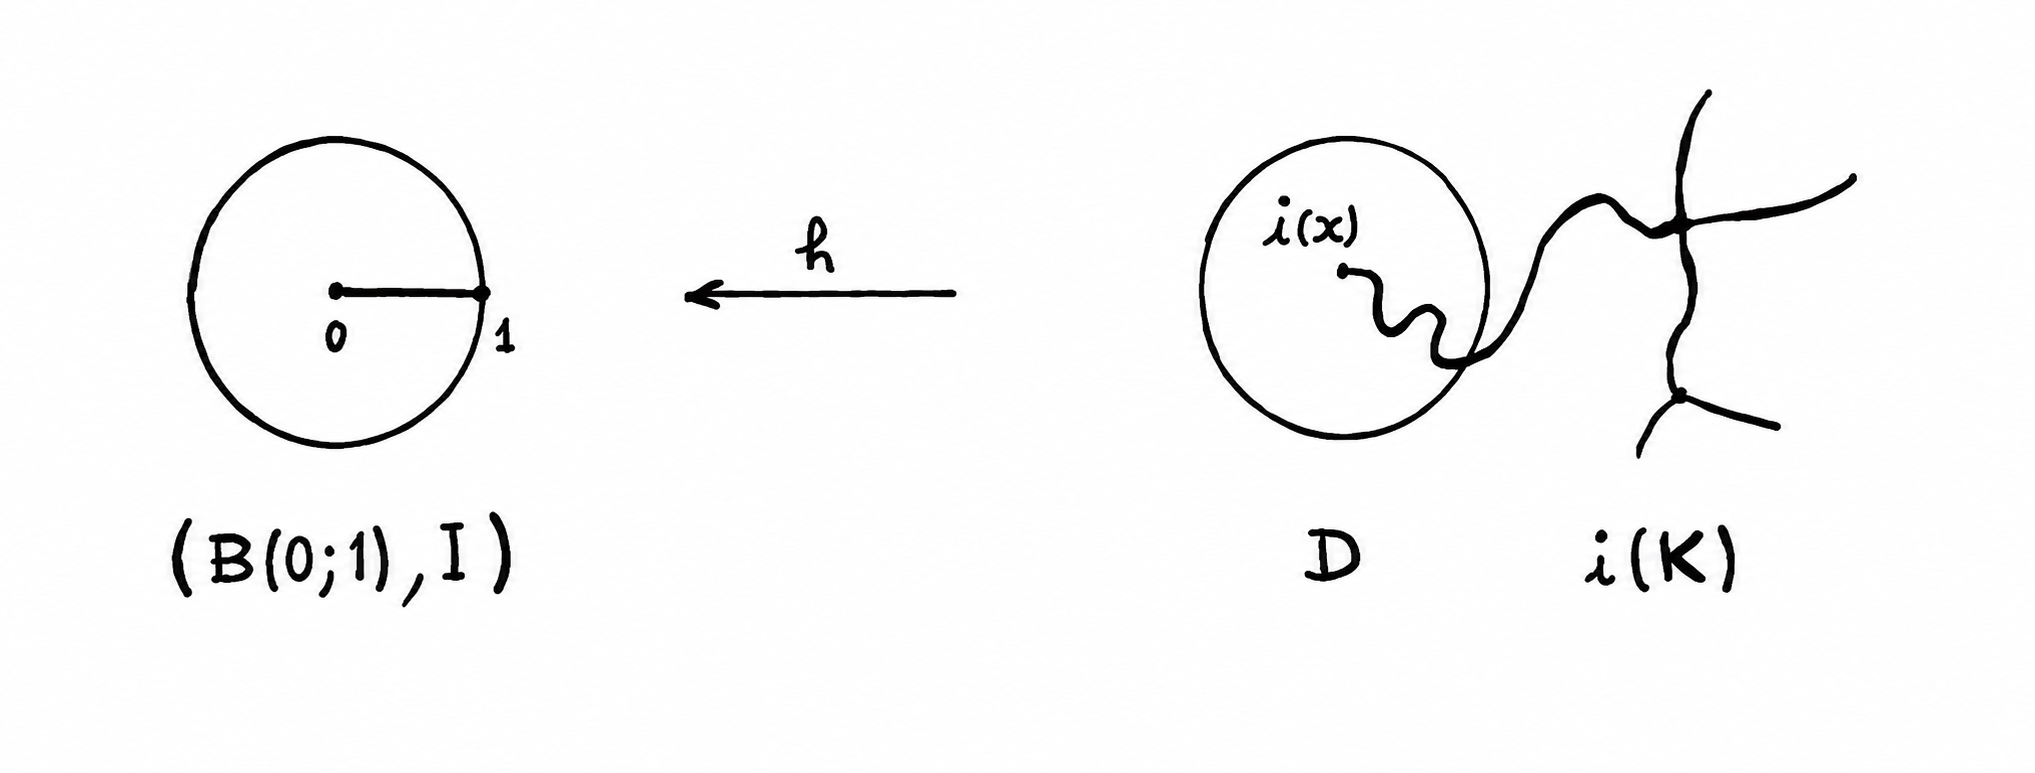
\includegraphics[width=130mm,scale=1]{figs/2.png}
\end{minipage}
\vskip .3cm
Soit $U$





order circulaire sur $\mathbb{S}^1$.
\vskip .3cm
\begin{minipage}{\linewidth}
    \centering
    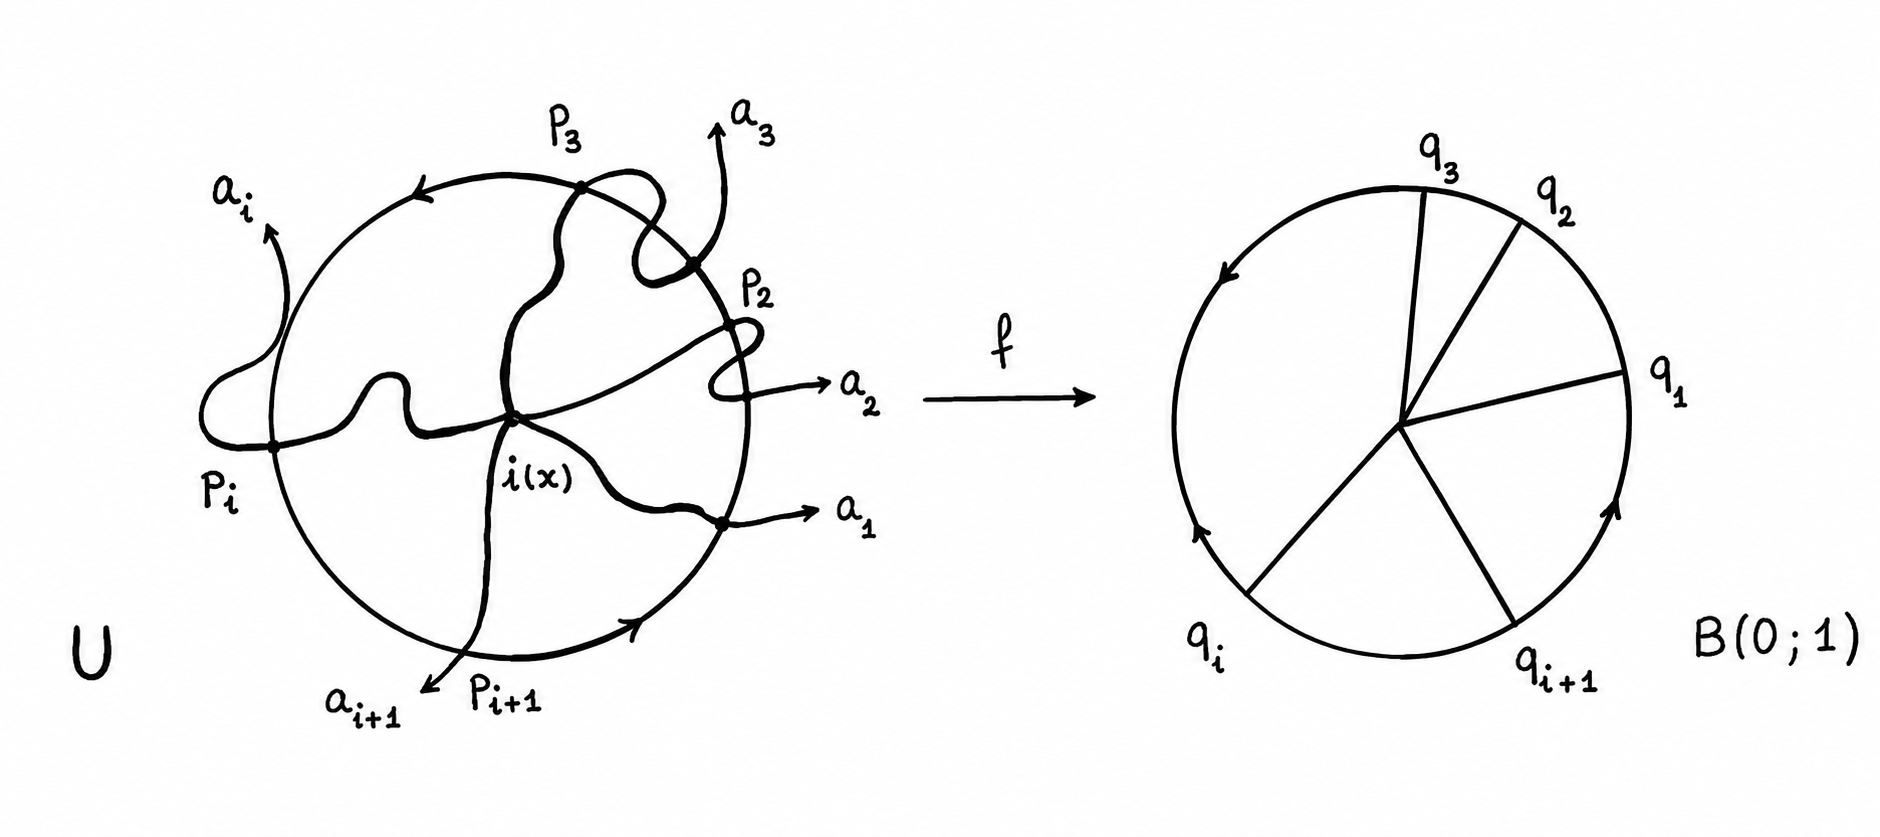
\includegraphics[width=130mm,scale=1]{figs/3.png}
\end{minipage}
\vskip .3cm
On note 



%%%%%%%%%%%%%%%%%%%%%%%%%%%%%%%%%%%%
\subsection*{3. Isotopie à un plongement P.L.. Problèmes d'intersections.}
\addcontentsline{toc}{subsection}{3. Isotopie à un plongement P.L.. Problèmes d'intersections}

{\bf 3.1}. ---



\vskip .3cm
{\bf 3.2}. ---



%%%%%%%%%%%%%%%%%%%%%%%%%%%%%%%%%%%%
\subsection*{4. Ordres circulaires induits par un plongement de 1-complexe.}
\addcontentsline{toc}{subsection}{4. Ordres circulaires induits par un plongement de 1-complexe}

{\bf 4.1}. ---


\vskip .3cm
{\bf 4.2}. ---



\vskip .3cm
{\bf 4.3}. ---



%%%%%%%%%%%%%%%%%%%%%%%%%%%%%%%%%%%%
\subsection*{5. Découpe d'un espace topologique suivant un fermé.}
\addcontentsline{toc}{subsection}{5. Découpe d'un espace topologique suivant un fermé}

{\bf 5.1}. ---

\vskip .3cm
{\bf 5.2}. ---


\vskip .3cm
{\bf 5.3}. ---


\vskip .3cm
{\bf 5.4}. ---


\vskip .3cm
{\bf 5.5}. --- Découpe et espace quotient.



\vskip .3cm
{\bf 5.6}. --- Fonctorialité de la découpe.

La découpe ne faisant intervenir dans sa définition que des éléments topologiques (transportables par homéomorphisme) définit de fa\c{c}on évidente un foncteur de la catégorie des couples $(X, K)$ ($X$~: espace topologique, $K$~: fermé de $X$) munie des homéomorphismes de couples, dans elle-même. (On pourrait même prendre pour morphismes de $(X, K)$ dans $(X', K')$ toutes les applications continues $f: X \to X'$ telles que $f^{-1}(K') = K$).

Ce foncteur induit de fa\c{c}on toute aussi évidente un foncteur $\Sigma$ de la catégorie des couples $(X, K)$ ($X$~: surface à bord généralisé, $K$~: 1-complexe contenu dans $\operatorname{int} X$) munie des homéomorphismes de couples, dans la catégorie des surfaces à bord généralisé (munie des homéomorphismes), et ceci grâce au théorème {\bf 5.4.2.}.

Si $(X, K)$ et $(X', K')$ sont deux objets de la première catégorie, et $h$ un homéomorphisme de $(X, K)$ sur $(X', K')$ on en déduit fonctoriellement un homéomorphisme $\Sigma (h)$ de $\Sigma (X, K)$ sur $\Sigma (X', K')$ (homéomorphisme qui induit un homéomorphisme entre les bords généralisés de $\Sigma (X, K)$ et $\Sigma (X', K')$).

N.B.~: dans tout la suite, on gardera les notations $\Sigma (X, K)$ et $\Sigma (h)$.


% End
